\section{Plots of Runge Kutta Method}

\begin{figure}[H]
  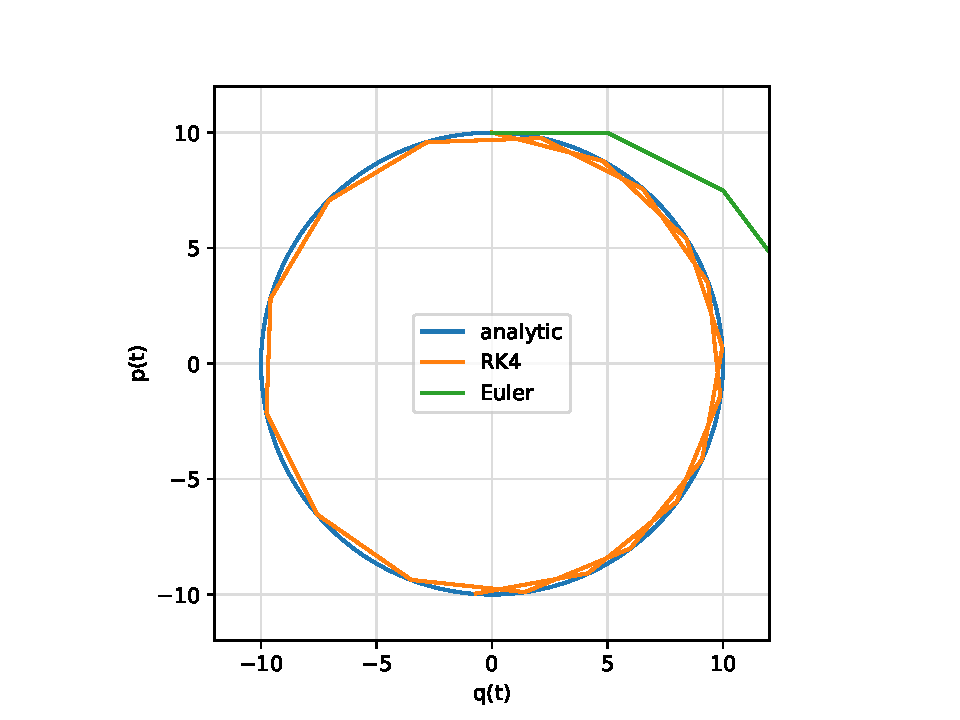
\includegraphics[width=\textwidth]{../python/rungekutta/plot-phasepath.pdf}
  \caption{This shows the evolution of the harmonic oscillator IVP given in the main section in phase space, solved by different mthods. Initial values are $u_0 = \{q_0, p_0\} = \{5, 0\} $. Stepsize \lstinline{deltat} = 0.4. One can see that the phase path calculated using Euler's method very quickly deviates from the analytical solution given by $ q(t) = \tfrac{p_0}{m}  \sin(t) + q_0 \cos(t)$ and $\tfrac{\mathrm{d}q}{\mathrm{d}t}(t) = \tfrac{p_0}{m} \cos(t) - q0 \sin(t)$. The RK4 solution instead remains one the circular path, hence is energy conserving.}
\end{figure}